\documentclass{jfrarticle}
\usepackage{amssymb}
\usepackage{mathtools}
\usepackage{tikz}
 \usepackage{bbm}
\usepackage{ dsfont }
\usepackage{hyperref}
\usepackage{ upgreek }
\usepackage{ stmaryrd }
 \usepackage[greek,english]{babel}
 % This handles the translation of unicode to latex:

 \usepackage{ucs}
 \usepackage[utf8x]{inputenc}
 \usepackage{autofe}
 % Some characters that are not automatically defined
 % (you figure out by the latex compilation errors you get),
 % and you need to define:

 \DeclareUnicodeCharacter{8988}{\ensuremath{\ulcorner}}
 \DeclareUnicodeCharacter{8989}{\ensuremath{\urcorner}}
 \DeclareUnicodeCharacter{8803}{\ensuremath{\overline{\equiv}}}
 \DeclareUnicodeCharacter{8718}{\ensuremath{\blacksquare}}
 \DeclareUnicodeCharacter{8759}{\ensuremath{::}}
 \DeclareUnicodeCharacter{955}{\ensuremath{\lambda}}
 \DeclareUnicodeCharacter{931}{\ensuremath{\Sigma}}
 \usepackage{fancyvrb}

 \DefineVerbatimEnvironment
   {code}{Verbatim}
   {} % Add fancy options here if you like.
\newcommand{\md}[1]{$\mathds{#1}$}

\title{A Formal Proof of the Undecidability of the Halting Problem}
\author{T. Altenkirch, Z. Yuan and A. Kaposi}
{THORSTEN ALTENKIRCH, ZONGZHE YUAN and AMBRUS KAPOSI\\School of Computer Science, University of Nottingham}

\begin{abstract}
We present here a formalisation of the proof of the undecidability of the Halting problem \cite{Turing} for the WHILE language introduced by Jones \cite{jones_computability_1997} using the Agda system \cite{agda}.  The main technical challenge is to implement and verify the self interpreter for the WHILE language. This work grew out of the final year project of the second author.
\end{abstract}
\begin{document}
\begin{bottomstuff}
T. Altenkirch was supported by the Engineering and Physical Sciences
Research Council (EPSRC) grant no. EPSRC grant EP/M016951/1 and USAF grant FA9550-16-1-0029.
\end{bottomstuff}
\maketitle 

\section{Introduction}
Alan Turing analysed and formalised the class of all computational procedure in 1936 \cite{turing_computable_1936} when the well-known computational model Turing Machine was introduced to the world.
Alan Turing has used the model of the Turing Machine to answer the question "Does a machine exist that can determine whether any arbitrary machine on its tape is 'circular'" and proved the undecidability of the Halting problem in 1936 as well \cite{turing_computable_1936}, which constitute the objective of this paper.\\
To prove the undecidability of the Halting problem, we must use a computational model that is Turing-equivalent to the Turing Machine in the thesis of the Church-Turing thesis \cite{copeland_church-turing_2002}.
To simplify, we choose a computational model that contains only one input, one output and a function mapping from the input to the output.
We choose some proper data structure D, which is in the form of binary tree, to represent the data of that computational model.
The function in that computational model is defined as a relation $\bullet \rightarrow \bullet \subseteq$ D $\times$ D that maps from the input to the output.
Then the concrete syntax and semantics for that computational model should be defined properly by using some proof assistant language and we choose Agda, an interactive theorem proof assistant language and dependently typed programming language \cite{agda} as the system in this proof.\\
Then we should construct the universal model following the thesis of Turing-completeness \cite{copeland_church-turing_2002}, which means for $f \in$ function, input and output $\in$ D as we defined and $f$(input) derives output, then the universal model $u$ has the property that $u(\lfloor f\rfloor \cdot $ input) derives output where $\lfloor f\rfloor$ is the code of function $f$ in the form of D and $\cdot$ is the concat symbol in the data structure D.\\
In order to prove the correctness of our universal computational model, we should define the concrete code method to code the function into the data structure D without ambiguity.
The first step in our process is to construct the interpretation step $s$ in the chosen system and prove the relation between the function \textit{f} and the interpretation \textit{s}.
The interpretation $s$ is defined as a stack machine: (Command,Stack,Variable) $\Rightarrow$ (Command',Stack',Variable') $\subseteq$ (D,D,D) $\times$ (D,D,D) which is a one-step relation between two triples.
The next proof is that if we have $f \in$ function, input and output $\in$ \textit{D} and $f$(input) derives output, then we can get $(\lfloor f\rfloor,\epsilon,$input)$ \Rightarrow^{*} (\epsilon,\epsilon,$output) where $\Rightarrow^{*}$ is multistep relationship of relation $\Rightarrow$.
The proof shows that the system we used here can interpret the function in our defined computational model.
Then by constructing the universal model properly, we can prove that the interpretation step in the system has correspondence to the interpretation in the universal model in which for $f \in$ function, input and output $\in$ D and $(\lfloor f\rfloor,\epsilon,$input)$ \Rightarrow^{*} (\epsilon,\epsilon,$output), the universal model $u$ has the property that $u(\lfloor f\rfloor \cdot $input) derives output.
The proof is inducted by the step of relation $\Rightarrow$.
Finally we can conclude that the computational model and the universal model has the correspondence that for $f \in$ function, input and output $\in$ D and $f$(input) derives output, then for the universal model $u$,  $u(\lfloor f\rfloor \cdot $input) derives output.\\
The proof of the undecidability of the Halting problem can be divided into three steps.
Initially we assume that there exists a program $h \in$ Program which has some properties: $\forall p \in$ Program and $\forall$ input $\in$ Data, if $p$ halts on input, then $h(\lfloor p\rfloor \cdot$ input) derives 1, else $h(\lfloor p\rfloor \cdot$ input) derives 0, which means $h$ decides the Halting problem.
Then we construct a program $m \in$ Program and feed $h$ to $m$ which means running $h$ inside $m$ and if the result of $h$ is 1, $m$ will loop forever, otherwise $m$ will halt immediately.
Then we run the program $m$ on its binary code $\lfloor m\rfloor$ which means inside $m$, $h$ will decide whether $m$ will halt on $\lfloor m\rfloor$ or not, which will end up in contradiction with the definition of $m$.
Finally we can conclude that $h$ doesn't exists by contradicting to our premise, which means there is no model that can decide the Halting problem, which otherwise means that the Halting problem is undecidable.

\section{Background}
\subsection{The Church-Turing Thesis}
The Church-Turing thesis is a hypothesis about the nature of computable functions \cite{church_unsolvable_1936}.
The thesis states that every effective computation can be carried out by a Turing Machine \cite{copeland_church-turing_2002}.
Turing gave the definition of his thesis as the LCMs [logical computing machines: Turing's expression for Turing Machines] can do anything, that can be described as "rule of thumb" or "purely mechanical" (Turing 1948:7.) \cite{copeland_church-turing_2002}.\\
The two basic concepts that related to this paper are the Turing-completeness and the Turing-equivalence.\\
\textit{Turing completeness} is the concept in the computability theory, such a computational model (for example a programming language, or recursive function) may satisfy Turing-completeness if and only if the model can be used to interpret any single-taped Turing Machine \cite{rogers_theory_1987}.\\
\textit{Turing equivalence} said that if two computational models can interpret each one by the other, then these two computational machine is called Turing-equivalence \cite{rogers_theory_1987}.\\
By the Church-Turing Thesis, any function that can be computed by some algorithm can be computed by a Turing Machine \cite{church_unsolvable_1936}, which means there are many computational models that is Turing equivalent to a Turing Machine \cite{copeland_church-turing_2002}.
Constructing and formalising a universal Turing Machine is quite complex, thus we can choose many other notions of effective (Turing-complete) computational model other than the Turing Machine:
\begin{itemize}
  \item Recursive functions as defined by Kleene \cite{yasuhara_recursive_1971}
  \item The lambda calculus approach to function definitions due to Church \cite{moggi_computational_1988}
  \item Random access machines \cite{cook_time-bounded_1972}
  \item Markov algorithms \cite{markov_2015}
\end{itemize}
Those computational models listed above have been proved to be Turing-equivalence to the Turing Machine and also have the property of Turing completeness.\\
\textit{Universal Turing Machine} is a Turing Machine that can interpret an arbitrary Turing Machine on arbitrary input \cite{universal_2016}. 
That is for $t \in$ TM, input and output $\in \Sigma^{*}$ ($\Sigma$ is the alphabet), and $t$(input) yields output, then the universal Turing Machine $u\in$ UTM has the property that $u(\lfloor t\rfloor \cdot$ input) yields output where $\lfloor t\rfloor$ is the code of Turing Machine $t$.

\subsection{Decidable and Non-Decidable}
In the area of computability, a set S is Recursive (Decidable) $\iff$ given a set D and S $\subseteq$ D, there is a function $f$ applies to the element $a \in$ D,
$f$ will return "true" if $a \in$ S and $f$ will return "false" if $a \notin$ S \cite{jones_computability_1997}.
Decidable set is closed under union, intersection, complement difference and Kleene star \cite{recursive_2015} circumstances.\\
A set S is Recursively Enumerable (Semi-Decidable) $\iff$ given a set D and S $\subseteq$ D, there is a function $f$ applies to the element $a \in$ D,
$f$ will return "true" if $a \in$ S and $f$ will return "false" or never terminate if $a \notin$ S which means no guarantee to terminate under the element $a \notin$ S \cite{jones_computability_1997}.
If a set S is recursively enumerable and the complement of S is also recursively enumerable, then set S is Recursive \cite{recursively_2015}.

\subsection{The Halting Problem}
In the area of computability theory, the Halting problem indicates that a given universal computing program (the model that is Turing-completeness \cite{jones_computability_1997}) 
may determine any other arbitrary computing program that would return the result on arbitrary input in a finite number of steps (a finite period of time), or would run forever \cite{halting_2015}.
That is, if there exists $h \in$ TM such that $\forall t \in$ TM, input $\in \Sigma^{*}$, if for $halt_{t}$(input), $h(\lfloor t\rfloor \cdot$ input) derives true and for $\neg halt_{t}$(input), $h(\lfloor t\rfloor \cdot$ input) derives false, then $h$ determining the Halting problem.\\
It is easily to prove that the Halting problem is semi-decidable \cite{halting_2015} because $\forall t \in$ TM, input $\in \Sigma^{*}$, if eventually $halt_{t}(input)$ then we can easily get the result.
However whether the Halting problem is decidable or not is interesting, and the aims to this paper is to prove the undecidable of the Halting problem.

\subsection{The WHILE language}
The WHILE language is a language that was just the right mixture of expressive power and simplicity, which provides the strict definitions of syntax and semantics and stays in the same level with Turing Machine model in terms of computing effectiveness (Turing-completeness) \cite{jones_computability_1997}. 
In addition, the data structure of WHILE treats the program as data object which can solve some rather complex missions that with the simplicity WHILE language can be simply used to prove many theorems and their behaviours \cite{jones_computability_1997}. 
By considering those several reasons, the project will focus on proving the undecidability of the Halting Problem in the model of WHILE language.
Thus, part of the definition, including the definition of WHILE language that was used in the project follows the definition in the paper \textit{Computability and Complexity: from a Programming Perspective} by \textit{Neil D. Jones} in 1997 \cite{jones_computability_1997}.

\subsection{Agda}
Agda, a dependent type language and an interactive proof assistant that
implements the Martin-Löf type theory \cite{van_oosten_homotopy_2014}, which can assist to develop a machine checked proof and formalise the proof of the Halting problem. 
Because the dependent type allow types to talk about values, the programs written by those languages can be encoded properties of values as types whose elements are proofs that the
property is true, which means that a dependently typed programming language can be used as a logic, and is needed to be integrated, not crash or non-terminate.
In addition, the mathematical proofs in Agda are written as structurally induction format, which are recursive functions that inducing on some inductive type argument which is equivalent to give mathematical proof by constructing some well-typed function that can finally terminate.
Therefore, Agda can be used as a framework to formalise formal logic systems and to prove the lemma which can be proved in mathematical ways.\\
We can use the key word \textbf{data} in Agda to define some inductive types, or more generally define some inductive families.
Here we define the basic type natural number as an example.
\begin{code}[fontsize=\small]
data ℕ : Set where
  zero : ℕ
  suc  : ℕ → ℕ
\end{code}
Then we can define the function \textit{plus} based on the natural number.
\begin{code}[fontsize=\small]
_+_ : ℕ → ℕ → ℕ
_+_ zero b = b
_+_ (suc a) b = suc (a + b)
\end{code}
Finally we can prove the \textit{associative	law} of our defined function by doing induction on the first argument, which is an inductive type in our definition.
\begin{code}[fontsize=\footnotesize]
suc-ok :  {a b : ℕ} → suc a + b ≡ suc (a + b)
suc-ok {zero} = refl
suc-ok {suc a} = cong suc refl

plus-asso : {a b c : ℕ} → (a + b) + c ≡ a + (b + c)
plus-asso {zero} = refl
plus-asso {suc a}{b}{c} = (suc a + b) + c
                        =⟨ cong (λ x → x + c) (suc-ok {a}{b}) ⟩
                        suc (a + b) + c
                        =⟨ suc-ok {a + b}{c} ⟩
                        (suc ((a + b) + c))
                        =⟨ cong suc (plus-asso {a}{b}{c}) ⟩
                        suc (a + (b + c))
                        ∎
\end{code}
Using Agda as the proof assistant language to this project has a lot of advantages that we can use Unicode characters while we write program in Agda, which let the proofs in Agda look similar to those logic proofs on paper and on textbooks.\\
The concept and those basic technique of Agda can be found in the book \textit{Dependently Typed Programming in Agda} by \textit{Ulf Norell and James Chapman} in 2009 \cite{norell_dependently_2009} and on the website \url{http://appserv.cs.chalmers.se/users/ulfn/wiki/agda.php} \cite{agda}.

\section{The WHILE Language in Agda}
Part of the definition, including the definition of WHILE language that was used here follows the definition in the paper \textit{Computability and Complexity: from a Programming Perspective} by \textit{Neil D. Jones} in 1997 \cite{jones_computability_1997}.
\subsection{Binary Tree Data Structure}
The language WHILE that computes with a binary tree data structure is built from a finite set. 
Thus we define that binary tree data structure $\mathds{D}$ with several related functions in Agda at first.
Initially, we should define the \textit{atoms} for the trees beforehand.
\textit{Atoms} mean small substances that can't be divided further into subparts.
However, the complexity in defining a large number of \textit{atoms} may make our proof become more complicated.
In fact, we can define only one \textit{atom} called \textit{nil} and because any other "atoms" that we presume to define can be constructed by combining different number of \textit{nil} in different order.
Thus, we define the data structure as:
\begin{code}[fontsize=\small]
data D : Set where
  dnil : D 
  _∙_  : D → D → D
\end{code}
And provide the approach to visit the first or the second element of an element in $\mathds{D}$.
\begin{code}[fontsize=\small]
dfst : D → D
dfst dnil = dnil
dfst (d₁ ∙ d₂) = d₁

dsnd : D → D
dsnd dnil = dnil
dsnd (d₁ ∙ d₂) = d₂
\end{code}

\subsection{Syntax}
The WHILE language is consist of three level definitions, the \textit{expression}, the \textit{command} and the \textit{program}, 
and the definition of the \textit{expression}, the \textit{command} and the \textit{program} can be found in page \textit{32} in the paper \textit{Computability and Complexity: from a Programming Perspective} by \textit{Neil D. Jones} in 1997 \cite{jones_computability_1997}.\\\\
The \textit{expression} is constructed in the form of binary tree, which has the same format of the data structure we defined previously.
A \textit{expression} is either the value of some variable, the \textit{atom} value which is the \textit{nil}, the first or the second value of another \textit{expression}, the combination of two \textit{expressions}, or the equality of two \textit{expressions}:\\
\textit{Expressions} \hspace{0.3cm}$\ni$\hspace{0.3cm} E, F\hspace{0.1cm} ::= X \hspace{0.98cm}(for X $\in$ Vars)\\
\indent\hspace{3.9cm}$|$ $d$\hspace{1cm} (for atom $d$, one atom \textit{nil} defined in Agda)\\
\indent\hspace{3.9cm}$|$ \textbf{cons} E F\\
\indent\hspace{3.9cm}$|$ \textbf{hd} E\\
\indent\hspace{3.9cm}$|$ \textbf{tl} E\\
\indent\hspace{3.9cm}$|$ \textbf{=?} E F\\
We define the data type of $\mathds{E}$ in Agda:
\begin{code}[fontsize=\small]
data E (n : ℕ) : Set where
  var  : Fin n → E n
  nil  : E n
  cons : E n → E n → E n
  hd   : E n → E n
  tl   : E n → E n
  _=?_ : E n → E n → E n
\end{code}
We use the member in a \textit{finite set} to represent the variables instead of variable names. 
For example \textit{Fin n} is a finite set that contains \textit{n} elements from \textit{zero} to $\underbrace{\mbox{\textit{suc (suc }} \dots \mbox{\textit{ suc (zero))}}}_{\textit{n - 1}}$.
Then we can directly use $\underbrace{\mbox{\textit{suc (suc }} \dots \mbox{\textit{ suc (zero))}}}_{\textit{k - 1}}$ to indicate the \textit{k}$_{th}$ variable's name (\textit{zero} is the first variable and so on).\\\\
A \textit{command} is either the assignment from some \textit{expressions} to some variables, or the sequence of two \textit{commands}, or the \textit{while} loop:\\
\textit{Commands} \hspace{0.35cm}$\ni$\hspace{0.35cm} C, D\hspace{0.1cm} ::= X := E\\
\indent\hspace{3.9cm}$|$ C \textbf{;} D\\
\indent\hspace{3.9cm}$|$ \textbf{while} E \textbf{do} C\\
And we define the data type of $\mathds{C}$ in Agda:
\begin{code}[fontsize=\small]
data C (n : ℕ) : Set where
  _:=_   : Fin n  → E n → C n
  _→→_ : C n → C n → C n
  while  : E n → C n → C n

\end{code}
The \textit{program} is consist of an \textit{input} variable which is the variable to store the \textit{input}, an \textit{output} variable which is the variable to store the final result:\\
Programs \hspace{0.5cm}$\ni$\hspace{0.4cm} P\hspace{0.6cm} ::= \textbf{read} X \textbf{;} C \textbf{;} \textbf{write} Y\\
And we define the same data type of $\mathds{P}$ in Agda:
\begin{code}[fontsize=\small]
data P (n : ℕ) : Set where
  prog : Fin n → C n → Fin n → P n
\end{code}

\subsection{Semantics}
To define the semantics of WHILE language, we must give a definition of the \textit{Partial Function} at first \cite{jones_computability_1997}:\\
Let \textit{A, B} be sets, a partial function \textit{g} is written as $g: A \rightarrow B_\bot$ and we said \textit{g} is effectively computable if there is an effective procedure such that for any $x \in A$:
\begin{itemize}
  \item The procedure eventually halts, yielding $g(x) \in B$, if $g(x)$ is defined;
  \item The procedure never halts, if $g(x)$ is undefined.
\end{itemize}
Then we can show that the program in WHILE can be used as a partial function from $\mathds{D}$ to $\mathds{D}_\bot$.\\\\
Initially, we define the \textit{environment} of the \textit{command}, written as $[x_1 \mapsto v_1, x_2 \mapsto v_2, \dots,x_n \mapsto v_n]$ to indicate the finite mapping function such that $s(x_i) = v_i$, where $v_i \in \mathds{D}$.
Then we use the notion $\sigma$ to indicate the \textit{environment} in WHILE that has type \textit{Store},
and for $p \in \mathds{P}$, $p$ $=$ read X; C; write Y, the initial store $\sigma_0^p$ is $[X \mapsto d, Y_1 \mapsto nil, \dots,Y_n \mapsto nil]$, and $\forall$ variable \textit{X} and \textit{Z} such that \textit{X} and \textit{Z} are variables in program \textit{p} and $X \neq Z$, then Z is in $Y_i$.\\
In Agda, we use the data type vector \textbf{Vec D n} to represent the store. Vector in Agda have the type:
\begin{code}
data Vec {a} (A : Set a) : ℕ → Set
\end{code}
which bind a list of certain type element with certain number of length.
Because the \textit{store} and the \textit{program} use the same $\textit{n}$ for both finite set of variables and their correspondence values,
the program is impossible to meet the condition that one variable hasn't been defined.\\\\
The definition of the semantics of WHILE language can be found in page \textit{40} in the paper \textit{Computability and Complexity: from a Programming Perspective} by \textit{Neil D. Jones} in 1997 \cite{jones_computability_1997}.\\\\
Then we define the evaluation function $\upvarepsilon$ with the type of $\mathds{E} \longrightarrow $ ($Store^p \rightarrow \mathds{D})$, 
which means for $e \in \mathds{E}$ and a given \textit{store} of program $\mathds{P}$ : $\sigma \in Store^{\mathds{P}}$, $\upvarepsilon \llbracket e \rrbracket \sigma = d \in \mathds{D}$.
Following the definition given by \textit{Neil D. Jones} in the paper\cite{jones_computability_1997}, the semantics of the evaluation function $\upvarepsilon$ in WHILE should be: for $e \in \mathds{E}$ and a given \textit{store} of program $\mathds{P}$, $\sigma \in Store^{\mathds{P}}$ $\upvarepsilon \llbracket e \rrbracket \sigma = d \in \mathds{D}$.\\
\indent\hspace{3cm}$\varepsilon \rrbracket$X$\rrbracket\sigma$ \hspace{1.5cm} = \hspace{0.3cm} $\sigma($X$)$\\
\indent\hspace{3cm}$\varepsilon \llbracket$d$\rrbracket\sigma$ \hspace{1.56cm} = \hspace{0.3cm} d\\
\indent\hspace{3cm}$\varepsilon \llbracket$cons E F$\rrbracket\sigma$ \hspace{0.4cm} = \hspace{0.3cm} $\varepsilon \llbracket$E$\rrbracket\sigma \centerdot \varepsilon \llbracket$F$\rrbracket\sigma$ \\
\indent\hspace{3cm}$\varepsilon \llbracket$hd E$\rrbracket\sigma$ \hspace{1.02cm} = \hspace{0.3cm} $\begin{cases} e & \mbox{if } \varepsilon \llbracket E \rrbracket\sigma = (e,f)\\ \mbox{nil} & \mbox{otherwise}\end{cases}$\\
\indent\hspace{3cm}$\varepsilon \llbracket$tl E$\rrbracket\sigma$ \hspace{1.2cm} = \hspace{0.3cm} $\begin{cases} f & \mbox{if } \varepsilon \llbracket E \rrbracket\sigma = (e,f)\\ \mbox{nil} & \mbox{otherwise}\end{cases}$\\
\indent\hspace{3cm}$\varepsilon \llbracket$=? E F$\rrbracket\sigma$ \hspace{0.6cm} = \hspace{0.3cm} $\begin{cases} \mbox{true} & \mbox{if } \varepsilon \llbracket E\rrbracket\sigma = \varepsilon \llbracket$F$\rrbracket\sigma\\ \mbox{false} & \mbox{otherwise}\end{cases}$\\
The Agda implementation of the evaluation function is defined as following:
\begin{code}[fontsize=\footnotesize]
eval : {n : ℕ} → E n → Vec D n → D
eval (var x) v = dlookup x v
eval nil v = dnil
eval (cons e₁ e₂) v = eval e₁ v ∙ eval e₂ v
eval (hd e) v = dhead (eval e v)
eval (tl e) v = dtail (eval e v)
eval (e₁ =? e₂) v with equalD? (eval e₁ v) (eval e₂ v)
eval (e₁ =? e₂) v | eq x = dnil ∙ dnil
eval (e₁ =? e₂) v | neq x = dnil

\end{code}
The execution of a \textit{command} in the program $\mathds{P}$ can be used as a function $f : \mathds{C} \times Store^{\mathds{P}} \times Store^{\mathds{P}}$.
However, because we can't guarantee that the execution of a \textit{command} will eventually halt and yield some output, the execution function should be a partial function $f : \mathds{C} \times Store^{\mathds{P}} \times Store^{\mathds{P}}_\bot$.
From this point of view, it is better to use a relation instead of a partial function to represent the execution of a \textit{command} \textit{c} $\in \mathds{C}$ as $c \vdash \sigma \rightarrow \sigma' \subseteq \mathds{C} \times Store^{\mathds{P}} \times Store^{\mathds{P}}$ where $\sigma'$ is the new \textit{environment} updated by the execution of \textit{command} \textit{c}
, following the definition given by \textit{Neil D. Jones} in the paper \cite{jones_computability_1997}\\
X\textbf{:=}E $\vdash\sigma \rightarrow \sigma[$X $\mapsto$ d$]$ \hspace{1.15cm}if \hspace{0.2cm} $\varepsilon \llbracket E \rrbracket \sigma = $ d\\
C\textbf{;}D $\vdash\sigma \rightarrow \sigma''$ \hspace{2.5cm}if \hspace{0.2cm} C $\vdash\sigma \rightarrow \sigma'$ and D $\vdash\sigma' \rightarrow \sigma''$\\
\textbf{while} E \textbf{do} C $\vdash\sigma \rightarrow \sigma''$ \hspace{0.95cm}if \hspace{0.2cm} C $\varepsilon \llbracket E \rrbracket \sigma \neq $ nil, C $\vdash\sigma \rightarrow \sigma'$,\\ \indent\hspace{7.5cm}\textbf{while} E \textbf{do} C $\vdash\sigma' \rightarrow \sigma''$\\
\textbf{while} E \textbf{do} C $\vdash\sigma \rightarrow \sigma$ \hspace{1.15cm}if \hspace{0.2cm} C $\varepsilon \llbracket E \rrbracket\sigma = $ nil\\
The Agda implementation of the execution relationship is defined as following:
\begin{code}[fontsize=\footnotesize]
data _⊢_⇒_ {n : ℕ} : C n → Vec D n  → Vec D n → Set where
  whilef : {e : E n}{c : C n}{env : Vec D n}
         → isNil (eval e env)
         → (while e c) ⊢ env ⇒ env
  whilet : {e : E n}{c : C n}{env₁ env₂ env₃ : Vec D n}
         → isTree (eval e env₁)
         → c ⊢ env₁ ⇒ env₂
         → (while e c) ⊢ env₂ ⇒ env₃
         → (while e c) ⊢ env₁ ⇒ env₃
  assign : {v : Fin n}{e : E n}{env : Vec D n}
         → (v := e) ⊢ env ⇒ (updateE v (eval e env) env)
  seq    : {c₁ c₂ : C n}{env₁ env₂ env₃ : Vec D n}
         → c₁ ⊢ env₁ ⇒ env₂
         → c₂ ⊢ env₂ ⇒ env₃
         → (c₁ →→ c₂) ⊢ env₁ ⇒ env₃

\end{code}
Similar to the definition of execution of $\mathds{C}$ in WHILE, the execution of program $\mathds{P}$ should also be defined as a relationship:\\
$\llbracket$$\bullet$$\rrbracket$$^{\mbox{WHILE}}$ : $\mathds{P}$ $\rightarrow$ ($\mathds{D}$ $\rightarrow$ $\mathds{D}$$_\perp$) defined for p = read X; C; write Y by:\\
$\llbracket$p$\rrbracket$$^{\mbox{WHILE}}$ = e if C $\vdash \sigma^p_0$(d)$ \rightarrow \sigma$ and $\sigma$(Y) = e\\
If there is no e such that $\llbracket$p$\rrbracket$ = e, then p loops on d; otherwise p terminates on d.\\
Following the definition, we define the partial relationship in Agda as following:
\begin{code}[fontsize=\small]
data ExecP {n : ℕ} : P n → D → D → Set where
  terminate : (x y : Fin n){c : C n}{env : Vec D n}{d : D}
            → c ⊢ (updateE x d initialVec) ⇒ env
            → ExecP (prog x c y) d (dlookup y env)
\end{code}
\subsection{Run WHILE in K Steps}
Even the execution of the \textit{command} \md{C} and the \textit{program} \md{P} are both a partial relationship, which means that we can't guarantee the eventual halt of the \textit{command} or the \textit{program} on some input(that is what we are proving),
we can still define the partial function that try to execute the \textit{command} \md{C} and \textit{program} \md{P} in \textit{k} steps.\\
Firstly we should define some data type to recored the execution step number of a given command.
\begin{code}[fontsize=\small]
record ResultCT {n : ℕ}(c : C n)(inp : Vec D n) : Set where
  field
    out  : Vec D n
    exe  : c ⊢ inp ⇒ out
    time : ℕ
\end{code}
Then we can construct the function to prove that one \textit{command} may be executed in \textit{k} stpes:
\begin{code}[fontsize=\small]
kStepC : {n : ℕ} → (k : ℕ) → (c : C n) → (inp : Vec D n) 
	→ (Maybe (ResultCT c inp))
kStepC = ?
\end{code}
The idea of that function is to do induction on the step number \textit{k} at first.
No \textit{command} can be run in \textit{zero} step.
Then the function will do induction on the \textit{command}.
The assignment step will only take \textit{1} step.
The steps that need to take relies on the sequence of two \textit{command} $c_1$ and $c_2$ will be the sum of steps that take on $c_1$ and the steps that costed on $c_2$.
Similarly in the \textit{while} loop, the \textit{command} will take \textit{zero} step if the \textit{expression} to the \textit{while} loop can be evaluated to \textit{false}.
It will cost steps that costed on $c$ and the continuous steps that costed on the following \textit{while} loop as the total steps to the \textit{command}.\\
Finally, if a command \textit{c} can be executed in \textit{k} steps, then a program \textit{p} = (read X; c; write Y) can also be executed in \textit{k} steps:
\begin{code}[fontsize=\small]
kStepP : {n : ℕ} → (time : ℕ) → (p : P n) → (inp : D) 
	→ (Maybe (Σ D (ExecP p inp)))
kStepP time (prog x c y) inp with kStepC time c (updateE x inp initialVec)
kStepP time (prog x c y) inp | just rc = just (dlookup y (ResultCT.out rc) , 
					       terminate x y (ResultCT.exe rc))
kStepP time (prog x c y) inp | nothing = nothing
\end{code}

\section{The Universal WHILE model}
Part of the definition, including the definition of the universal WHILE model that was used here follows the definition in the paper \textit{Computability and Complexity: from a Programming Perspective} by \textit{Neil D. Jones} in 1997 \cite{jones_computability_1997}.
\subsection{Interpretation of the WHILE program}
In order to construct the universal WHILE model in Agda later, we must define the method to code a program into form of \md{D} in order to feed the program as the input to the universal WHILE program later.
It is important to define the operator $\bullet$ of our data structure \md{D} with no association, which would avoid ambiguity.\\
Following the definition "Let \{ :=, ;, while, var, quote, cons, hd, tl, =?, nil \} denote 10 distinct elements of \md{D}, and let \{ dohd, dotl, docons, doasgn, dowh, do=? \} denote 6 more values in \md{D}" in page \textit{67} in the paper \textit{Computability and Complexity: from a Programming Perspective} by \textit{Neil D. Jones} \cite{jones_computability_1997}, we define some constants to indicate some distinct elements of \md{D}, which would represent the \textit{program} in the form of \md{D}.\\
Then we defined the function that map the \textit{program} to \md{D}: $code \in \mathds{P} \times \mathds{D}$.
The mapping function from the WHILE program to WHILE data is defined as:\\
\indent\hspace{3cm}\underline{read V$_i$; C; write V$_j$}\hspace{0.55cm} = \hspace{0.5cm} ((vari)\underline{C}(varj))\\\\
\indent\hspace{3cm}\underline{C; D}\hspace{3cm} = \hspace{0.5cm} (;\underline{CD})\\
\indent\hspace{3cm}\underline{while E do C}\hspace{1.7cm} = \hspace{0.5cm} (while\underline{EC})\\
\indent\hspace{3cm}\underline{V$_i$:= E}\hspace{2.6cm} = \hspace{0.5cm} (:=(vari)\underline{E})\\\\
\indent\hspace{3cm}\underline{V$_i$}\hspace{3.3cm} = \hspace{0.5cm} (vari)\\
\indent\hspace{3cm}\underline{d}\hspace{3.5cm} = \hspace{0.5cm} (quoted)\\
\indent\hspace{3cm}\underline{cons E F}\hspace{2.3cm} = \hspace{0.5cm} (cons\underline{EF})\\
\indent\hspace{3cm}\underline{hd E}\hspace{2.95cm} = \hspace{0.5cm} (hd\underline{E})\\
\indent\hspace{3cm}\underline{tl E}\hspace{3.1cm} = \hspace{0.5cm} (tl\underline{E})\\
\indent\hspace{3cm}\underline{=? E F}\hspace{2.55cm} = \hspace{0.5cm} (=?\underline{EF})\\
Initially we should define the function that code the \textit{expression} into \md{D}.
The definition of that function in Agda following the the definition above:
\begin{code}[fontsize=\small]
codeE : {n : ℕ} → E n → D
codeE (var x) = dvar ∙ dftod x
codeE nil = dquote ∙ dnil
codeE (cons e₁ e₂) = dcons ∙ (codeE e₁ ∙ codeE e₂)
codeE (hd e) = dhd ∙ codeE e
codeE (tl e) = dtl ∙ codeE e
codeE (e₁ =? e₂) = d=? ∙ (codeE e₁ ∙ codeE e₂)

\end{code}
Then we should define the function that code the \textit{command} into \md{D}.
The definition of that function in Agda following the the definition above:
\begin{code}[fontsize=\small]
codeC : {n : ℕ} → C n → D
codeC (x := e) = d:= ∙ ((dvar ∙ dftod x) ∙ codeE e)
codeC (c₁ →→ c₂) = d→→ ∙ (codeC c₁ ∙ codeC c₂)
codeC (while e c) = dwhile ∙ (codeE e ∙ codeC c)

\end{code}
Finally we should define the function that code the \textit{program} into \md{D}.
The definition of that function in Agda following the the definition above:
\begin{code}[fontsize=\small]
codeP : {n : ℕ} → P n → D
codeP {n} (prog x c y) = (dvar ∙ dftod x) ∙
                         (codeC c ∙
                         (dvar ∙ dftod y))
\end{code}
In the later version, I also add the number of variables of the program to the result of coding in order to allow the universal WHILE program can interpret any WHILE program with arbitrary variables in the future work.\\\\
Beyond the coding method that maps the \textit{program} to \md{D}, I also define the function that decode the \md{D} and map it to the \textit{program}.
However because the function \textit{decode} is a partial function, sometimes it may cause decoding fail because the input \md{D} doesn't follow the format of the program.
\begin{code}[fontsize=\small]
decodeE : {n : ℕ} → D → Maybe (E n)
decodeE = ?

decodeC : {n : ℕ} → D → Maybe (C n)
decodeC = ?

decodeP : D → Maybe (Σ ℕ P)
decodeP = ?
\end{code}
\subsection{The Universal WHILE model}
Initially we should define the 8 variables in the WHILE language: \{PD, P, C, Cd, St, V1, W, Z\}.\\
Then we should define some syntax sugar such as \textit{if} and \textit{if-else}:
\begin{code}[fontsize=\footnotesize]
if8 : E 8 → C 8 → C 8
if8 e c = (Z := e) →→ while (var Z) ((Z := nil) →→ c)

if-else8 : E 8 → C 8 → C 8 → C 8
if-else8 e c₁ c₂ = (Z := e) →→
                   (W := cons nil nil) →→
                   ((while (var Z)
                           ((Z := nil) →→
                           ((W := nil) →→
                           c₁))) →→
                   (while (var W)
                          ((W := nil) →→
                          c₂)))
\end{code}
Finally we should define the universal WHILE program.
Here we firstly define the universal WHILE program that can interpret other WHILE program which has only one variable.
The universal WHILE program which could interpret the WHILE program of $1$ variable is defined as:
\begin{code}[fontsize=\small]
read PD;             (* Input (p.d) *)
  P := hd PD;        (* P = ((var 1) C (var 1)) *)
  C := hd (tl P)     (* C = hd tl p program code is C *)
  Cd := cons C nil;  (* Cd = (c.nil), Code to execute is c *)
  St := nil;         (* St = nil, Stack empty *)
  Vl := tl PD;       (* Vl = d Initial value of var.*)
  while Cd do STEP;  (* do while there is code to execute *)
write Vl;
\end{code}
Where the \textit{STEP} is the Macro that interprets the program.
Then the program is defined in Agda as:
\begin{code}[fontsize=\small]
universalI : P 8
universalI = prog PD ((Pp := hd (var PD))
                     →→
                     (Cc := hd (tl (var Pp)))
                     →→
                     (Cd := cons (var Cc) nil)
                     →→
                     (St := nil)
                     →→
                     (V1 := tl (var PD))
                     →→
                     (while (var Cd) STEP-I))
                  V1

\end{code}
When we are interpreting a WHILE program which has only one variable, we can easily define a stack machine as a Macro based on three variables: \textit{Cd} which is the \textit{command}, \textit{St} which is the stack and \textit{V1} which is the only one variable.
Here we define the syntax sugar \textit{cons$^{*}$} as \textit{cons$^{*}$} \textit{A B C} = \textit{cons} \textit{A} (\textit{cons B C}). 
Then we could rewrite [Cd, St] by:\\
\indent\hspace{0.5cm}[((quote D)$\cdot$Cr), St]\hspace{1.55cm} $\Rightarrow$ \hspace{0.5cm} [Cr, cons D St]\\
\indent\hspace{0.5cm}[((var 1)$\cdot$Cr), St]\hspace{2.1cm} $\Rightarrow$ \hspace{0.5cm} [Cr, cons V1 St]\\
\indent\hspace{0.5cm}[((hd E)$\cdot$Cr), St]\hspace{2.15cm} $\Rightarrow$ \hspace{0.5cm} [cons$^{*}$ E dohd Cr, Sr]\\
\indent\hspace{0.5cm}[(dohd$\cdot$Cr), (T$\cdot$Sr)]\hspace{1.7cm} $\Rightarrow$ \hspace{0.5cm} [Cr, cons (hd T) St]\\
\indent\hspace{0.5cm}[((tl E)$\cdot$Cr), St]\hspace{2.35cm} $\Rightarrow$ \hspace{0.5cm} [cons$^{*}$ E dotl Cr, St]\\
\indent\hspace{0.5cm}[(dotl$\cdot$Cr), (T$\cdot$Sr)]\hspace{1.9cm} $\Rightarrow$ \hspace{0.5cm} [Cr, cons (tl T) Sr]\\
\indent\hspace{0.5cm}[((cons E$_1$ E$_2$)$\cdot$Cr), St]\hspace{1.1cm} $\Rightarrow$ \hspace{0.5cm} [cons$^{*}$ E$_1$ E$_2$ docons Cr, St]\\
\indent\hspace{0.5cm}[(docons$\cdot$Cr), (U$\cdot$(T$\cdot$Sr))]\hspace{0.7cm} $\Rightarrow$ \hspace{0.5cm} [Cr, cons (cons T U) Sr]\\
\indent\hspace{0.5cm}[((=? E$_1$ E$_2$)$\cdot$Cr), St]\hspace{1.35cm} $\Rightarrow$ \hspace{0.5cm} [cons$^{*}$ E$_1$ E$_2$ do=? Cr, St]\\
\indent\hspace{0.5cm}[(do=?$\cdot$Cr), (U$\cdot$(T$\cdot$Sr))]\hspace{1cm} $\Rightarrow$ \hspace{0.5cm} [Cr, cons (=? T U) St]\\
\indent\hspace{0.5cm}[((; C$_1$ C$_2$)$\cdot$Cr), St]\hspace{1.8cm} $\Rightarrow$ \hspace{0.5cm} [cons$^{*}$ C$_1$ C$_2$ Cr, St]\\
\indent\hspace{0.5cm}[((:= (var 1) E)$\cdot$Cr), St]\hspace{0.9cm} $\Rightarrow$ \hspace{0.5cm} [cons$^{*}$ E doasgn Cr, St]\\
\indent\hspace{0.5cm}[(doasgn$\cdot$Cr), (W$\cdot$Sr)]\hspace{1.35cm} $\Rightarrow$ \hspace{0.5cm} \{Cd := Cr, St := Sr; V1 := W\}\\
\indent\hspace{0.5cm}[((while E C)$\cdot$Cr), St]\hspace{1.35cm} $\Rightarrow$ \hspace{0.5cm} [cons$^{*}$ E dowh (while E C) Cr, St]\\
\indent\hspace{0.5cm}[(dowh$\cdot$((while E C)$\cdot$Cr)), (nil$\cdot$Sr)]\hspace{0.85cm} $\Rightarrow$ \hspace{0.5cm} [Cr, Sr]\\
\indent\hspace{0.5cm}[(dowh$\cdot$((while E C)$\cdot$Cr)), ((A$\cdot$B)$\cdot$Sr)]\hspace{0.3cm} $\Rightarrow$ \hspace{0.5cm} [cons$^{*}$ C (while E C) Cr, Sr]\\
\indent\hspace{0.5cm}[nil, St]\hspace{3.9cm} $\Rightarrow$ \hspace{0.5cm} [nil, St]\\
Initially we define the data relationship $(Cd,St,V1)\Rightarrow(Cd',St',V1')$ $\in$  $(\mathds{D},\mathds{D},\mathds{D})\times (\mathds{D},\mathds{D},\mathds{D})$ as a one step relationship.
Then we define the interpretation step following the definition using Agda:
\begin{code}[fontsize=\scriptsize]
data _⇒_ : D × D × D → D × D × D → Set where
  equote  : (d Cr St V1 : D)
            → < (dquote ∙ d) ∙ Cr , St , V1 >
            ⇒ < Cr , d ∙ St , V1 >
  evar1   : (Cr St V1 : D)
            → < (dvar ∙ dftod {1} zero) ∙ Cr , St , V1 >
            ⇒ < Cr , V1 ∙ St , V1 >
  ehd     : (E Cr St V1 : D)
            → < (dhd ∙ E) ∙ Cr , St , V1 >
            ⇒ < E ∙ (dohd ∙ Cr) , St , V1 >
  edohd   : (T Cr St V1 : D)
            → < dohd ∙ Cr , T ∙ St , V1 >
            ⇒ < Cr , (dfst T) ∙ St , V1 >
  etl     : (E Cr St V1 : D)
            → < (dtl ∙ E) ∙ Cr , St , V1 >
            ⇒ < E ∙ (dotl ∙ Cr) , St , V1 >
  edotl   : (T Cr St V1 : D)
            → < dotl ∙ Cr , T ∙ St , V1 >
            ⇒ < Cr , (dsnd T) ∙ St , V1 >
  econs   : (E₁ E₂ Cr St V1 : D)
            → < (dcons ∙ (E₁ ∙ E₂)) ∙ Cr , St , V1 >
            ⇒ < E₁ ∙ (E₂ ∙ (docons ∙ Cr)) , St , V1 >
  edocons : (U T Cr St V1 : D)
            → < docons ∙ Cr , U ∙ (T ∙ St) , V1 >
            ⇒ < Cr , (T ∙ U) ∙ St , V1 >
  e=?     : (E₁ E₂ Cr St V1 : D)
            → < (d=? ∙ (E₁ ∙ E₂)) ∙ Cr , St , V1 >
            ⇒ < E₁ ∙ (E₂ ∙ (do=? ∙ Cr)) , St , V1 >
  edo=?   : (U T Cr St V1 : D)
            → < do=? ∙ Cr , U ∙ (T ∙ St) , V1 >
            ⇒ < Cr , (dequal T U) ∙ St , V1 >
  e→→     : (C₁ C₂ Cr St V1 : D)
            → < (d→→ ∙ (C₁ ∙ C₂)) ∙ Cr , St , V1 >
            ⇒ < C₁ ∙ (C₂ ∙ Cr) , St , V1 >
  e:=     : (E Cr St V1 : D)
            → < (d:= ∙ ((dvar ∙ dftod {1} zero) ∙ E)) ∙ Cr , St , V1 >
            ⇒ < E ∙ (doasgn ∙ Cr) , St , V1 >
  edoasgn : (W Cr St V1 : D)
            → < doasgn ∙ Cr , W ∙ St , V1 >
            ⇒ < Cr , St , W >
  ewhile  : (E C Cr St V1 : D)
            → < (dwhile ∙ (E ∙ C)) ∙ Cr , St , V1 >
            ⇒ < E ∙ (dowh ∙ ((dwhile ∙ (E ∙ C)) ∙ Cr)) , St , V1 >
  edowhf  : (E C Cr St V1 : D)
            → < dowh ∙ ((dwhile ∙ (E ∙ C)) ∙ Cr) , dnil ∙ St , V1 >
            ⇒ < Cr , St , V1 >
  edowht  : (E C X Y Cr St V1 : D)
            → < dowh ∙ ((dwhile ∙ (E ∙ C)) ∙ Cr) , (X ∙ Y) ∙ St , V1 >
            ⇒ <  C ∙ ((dwhile ∙ (E ∙ C)) ∙ Cr)  , St , V1 >
  enil    : (St V1 : D) → < dnil , St , V1 > ⇒ < dnil , St , V1 >
\end{code}
Furthermore, we define the multi-steps relationship $(Cd,St,V1)\Rightarrow^*(Cd',St',V1')$ $\in$  $(\mathds{D},\mathds{D},\mathds{D})\times (\mathds{D},\mathds{D},\mathds{D})$.
\begin{code}[fontsize=\small]
data _⇒*_ : D × D × D → D × D × D → Set where
  id   : (Cr St V1 : D) → < Cr , St , V1 > ⇒* < Cr , St , V1 >
  seq  : (Cr₁ Cr₂ Cr₃ St₁ St₂ St₃ V1₁ V1₂ V1₃ : D)
         → < Cr₁ , St₁ , V1₁ > ⇒  < Cr₂ , St₂ , V1₂ >
         → < Cr₂ , St₂ , V1₂ > ⇒* < Cr₃ , St₃ , V1₃ >
         → < Cr₁ , St₁ , V1₁ > ⇒* < Cr₃ , St₃ , V1₃ >
\end{code}
We should proof the associative of relation $\Rightarrow^*$.
\begin{code}[fontsize=\small]
  ⇒*-m : (Cr₁ Cr₂ Cr₃ St₁ St₂ St₃ V1₁ V1₂ V1₃ : D)
              → < Cr₁ , St₁ , V1₁ > ⇒* < Cr₂ , St₂ , V1₂ >
              → < Cr₂ , St₂ , V1₂ > ⇒* < Cr₃ , St₃ , V1₃ >
              → < Cr₁ , St₁ , V1₁ > ⇒* < Cr₃ , St₃ , V1₃ >
  ⇒*-m = ?
  ⇒*-b : (Cr₁ Cr₂ Cr₃ St₁ St₂ St₃ V1₁ V1₂ V1₃ : D)
              → < Cr₁ , St₁ , V1₁ > ⇒* < Cr₂ , St₂ , V1₂ >
              → < Cr₂ , St₂ , V1₂ > ⇒  < Cr₃ , St₃ , V1₃ >
              → < Cr₁ , St₁ , V1₁ > ⇒* < Cr₃ , St₃ , V1₃ >
  ⇒*-b = ?
\end{code}
Then we can prove the relationship between the WHILE language and the interpretation step on \textit{expression e}, such that for $E \in \mathds{E}$, $\upvarepsilon \llbracket E \rrbracket [V1 \mapsto d] = d_e$, then $((codeE\cdot Cr),St,d)\Rightarrow^*(Cr,(d_e\cdot St),d)$, and the proof is inducted by the \textit{expression}.
\begin{code}[fontsize=\small]
⇒*e : (e : E 1) → (d₁ d₂ Cr St : D)
       → eval e (updateE zero d₁ initialVec) ≡ d₂
       → < codeE e ∙ Cr , St , d₁ > ⇒* < Cr , d₂ ∙ St , d₁ >
⇒*e = ?
\end{code}
After that, we can prove the relationship between the WHILE language and the interpretation step on execution of \textit{command}, such that for $C \in \mathds{C}$, $C \vdash [V1 \mapsto d_1] \Rightarrow [V1 \mapsto d_2]$, then $((codeC$ $C\cdot Cr),St,d_1)\Rightarrow^*(Cr,St,d_2)$, and the proof is inducted by the \textit{command}.\\
As we know the \textit{command} can be the form of \textit{while} loop, and when we do induction on the \textit{while} loop \textit{while e c}, the \textit{command} to the subproblem will also be \textit{while e c}.
The only change to the subproblem is the \textit{environment}.
However, those will violate the \textit{termination checker} in Agda, which causes the \textit{termination checking fail} error.
In Agda, when we do induction on some inductive variables, the variables in the subproblem should be 'smaller' than the variables in the original problem, in which way Agda will treat the function as that could be terminated eventually.
Even the \textit{command} can meet the situation of \textit{infinite while loop}, the type to the relation is consistent, and the proof function should eventually be terminated.
Thus, we need some auxiliary data type to indicate that after one step, the \textit{command} to the subproblem is definitely smaller than the \textit{command} to the original problem.
Here we called the new data type \textit{call tree}.
\begin{code}[fontsize=\small]
data callTree : Set where
  cnil : callTree 
  cons : callTree → callTree → callTree
\end{code}
The \textit{assignment} in the \textit{command} only costs one  step, which is the \textit{cnil} in the \textit{call tree}.
The \textit{sequence} ($seq$ $c_1$ $c_2$) costs $callTree_1$ for $c_1$ and $callTree_2$ for $c_2$.
The \textit{while} loop (\textit{while e c}) costs $callTree_1$ for $c$ and $callTree_2$ for the consequence (\textit{while e c}).
Compare to ($cons$ $callTree_1$ $callTree_2$), $callTree_2$ is smaller without doubt.
Thus, the \textit{command} to the subproblem is definitely smaller than the \textit{command} to the original problem.
And because both \textit{callTree} and \md{D} has the form of binary tree, we use \md{D} instead of \textit{callTree}, and the proof function should be:
\begin{code}[fontsize=\small]
loop-ct : {n : ℕ}{c : C n}{env₁ env₂ : Vec D n} → c ⊢ env₁ ⇒ env₂ → D
loop-ct (whilef x) = dnil
loop-ct (whilet x p p₁) = (loop-ct p) ∙ (loop-ct p₁)
loop-ct assign = dnil
loop-ct (seq p p₁) = (loop-ct p) ∙ (loop-ct p₁)

⇒*proof : {t : D} → (c : C 1) → (d₁ d₂ Cr St : D) → (out : Vec D 1)
       → (p : c ⊢ updateE zero d₁ initialVec ⇒ out)
       → dlookup zero out ≡ d₂
       → loop-ct p ≡ t
       → < codeC c ∙ Cr , St , d₁ > ⇒* < Cr , St , d₂ >
⇒*proof = ?
\end{code}
In the proof, we initially do induction on \textit{command}.
For the case of \textit{while} loop, we do induction on the '\textit{callTree}' $t$ to indicate that the execution of \textit{while e c} in the subproblem is definitely 'smaller' than that in the original problem. 
\begin{code}[fontsize=\small]
⇒*ok : (c : C 1) → (d₁ d₂ Cr St : D) → (out : Vec D 1)
       → c ⊢ updateE zero d₁ initialVec ⇒ out
       → dlookup zero out ≡ d₂
       → < codeC c ∙ Cr , St , d₁ > ⇒* < Cr , St , d₂ >
⇒*ok c d₁ d₂ Cr St out p q = ⇒*proof {loop-ct p} c d₁ d₂ Cr St out p q refl
\end{code}
This proof shows that the execution of the \textit{command} in WHILE language has relationship with the relation $\Rightarrow$, which means that one step of execution of \textit{command} is corresponding to the multi-step $\Rightarrow^*$ accordingly, which is the interpretation of WHILE program in \textit{Agda}.\\\\
Then we define the real universal WHILE program.
The most important part is the \textit{STEP} Macro.
Before we defining the Macro, we should define those sixteen constants in the form of \md{E}, and we can define \textit{STEP} as a \textit{command} in Agda:
\begin{code}[fontsize=\small]
STEP-I : C 8
STEP-I =  ?
\end{code}
We don't have pattern match in WHILE language, thus we use a bunch of \textit{if-else} we defined previously to define the \textit{STEP} macro in the form of \textit{command} in WHILE language.\\ 
Then we can prove that the interpretation holds by Agda has one step correspondence with the Macro \textit{STEP}.
That is, if $(Cd,St,V1)\Rightarrow(Cd',St',V1')$, then \textit{STEP} $\vdash [\dots, Cd, St, V1, \dots] \Rightarrow [\dots, Cd', St', V1', \dots]$:
\begin{code}[fontsize=\footnotesize]
c-h : {Pd P C : D}(d₁ d₂ Cr₁ Cr₂ St₁ St₂ : D) 
      → < Cr₁ , St₁ , d₁ > ⇒ < Cr₂ , St₂ , d₂ >
      → STEP-I ⊢ (Pd ∷ P ∷ C ∷ Cr₁ ∷ St₁ ∷ d₁ ∷ dnil ∷ dnil ∷ [])
               ⇒ (Pd ∷ P ∷ C ∷ Cr₂ ∷ St₂ ∷ d₂ ∷ dnil ∷ dnil ∷ [])
c-h d₁ .d₁ .((dquote ∙ d) ∙ Cr) Cr St .(d ∙ St) (equote d .Cr .St .d₁) = case1
c-h d₁ .d₁ .((dvar ∙ dnil) ∙ Cr) Cr St .(d₁ ∙ St) (evar1 .Cr .St .d₁) = case2
c-h d₁ .d₁ .((dhd ∙ E) ∙ Cr) .(E ∙ (dohd ∙ Cr)) St .St (ehd E Cr .St .d₁) = case3
c-h d₁ .d₁ .(dohd ∙ Cr) Cr .(T ∙ St) .(dfst T ∙ St) (edohd T .Cr St .d₁) = case4
c-h d₁ .d₁ .((dtl ∙ E) ∙ Cr) .(E ∙ (dotl ∙ Cr)) St .St (etl E Cr .St .d₁) = case5
c-h d₁ .d₁ .(dotl ∙ Cr) Cr .(T ∙ St) .(dsnd T ∙ St) (edotl T .Cr St .d₁) = case6
c-h d₁ .d₁ .((dcons ∙ (E₁ ∙ E₂)) ∙ Cr) .(E₁ ∙ (E₂ ∙ (docons ∙ Cr))) 
					St .St (econs E₁ E₂ Cr .St .d₁) = case7
c-h d₁ .d₁ .(docons ∙ Cr) Cr .(U ∙ (T ∙ St)) .((T ∙ U) ∙ St) 
						(edocons U T .Cr St .d₁) = case8
c-h d₁ .d₁ .((d=? ∙ (E₁ ∙ E₂)) ∙ Cr) .(E₁ ∙ (E₂ ∙ (do=? ∙ Cr))) St .St 
						(e=? E₁ E₂ Cr .St .d₁) = case9
c-h d₁ .d₁ .(do=? ∙ Cr) Cr .(U ∙ (T ∙ St)) .(_ ∙ St) 
						(edo=? U T .Cr St .d₁) = case10
c-h d₁ .d₁ .((d→→ ∙ (C₁ ∙ C₂)) ∙ Cr) .(C₁ ∙ (C₂ ∙ Cr)) St .St 
						(e→→ C₁ C₂ Cr .St .d₁) = case11
c-h d₁ .d₁ .((d:= ∙ ((dvar ∙ dnil) ∙ E)) ∙ Cr) .(E ∙ (doasgn ∙ Cr)) St .St 
							(e:= E Cr .St .d₁) = case12
c-h d₁  d₂ .(doasgn ∙ Cr) Cr .(d₂ ∙ St) St (edoasgn .d₂ .Cr .St .d₁) = case13
c-h d₁ .d₁ .((dwhile ∙ (E ∙ C₁)) ∙ Cr) .(E ∙ (dowh ∙ ((dwhile ∙ (E ∙ C₁)) ∙ Cr))) 
					St .St (ewhile E C₁ Cr .St .d₁) = case14
c-h d₁ .d₁ .(dowh ∙ ((dwhile ∙ (E ∙ C₁)) ∙ Cr)) Cr .(dnil ∙ St) St 
						(edowhf E C₁ .Cr .St .d₁) = case15
c-h d₁ .d₁ .(dowh ∙ ((dwhile ∙ (E ∙ C₁)) ∙ Cr)) .(C₁ ∙ ((dwhile ∙ (E ∙ C₁)) ∙ Cr)) 
			.((X ∙ Y) ∙ St) St (edowht E C₁ X Y Cr .St .d₁) = case16
c-h d₁ .d₁ .dnil .dnil St .St (enil .St .d₁) = case17
\end{code}
We do induction on Cr$_1$ at first.
The proof has been divided into several files because in order to make the compilation of that proof faster in Agda, we must provide the \textit{environment} to each step of the execution of the \textit{command} \textit{STEP-I}, which will take up a lot of space. 
\begin{code}[fontsize=\scriptsize]
case1 : {d St Cr d₁ C P Pd : D} 
	→ STEP-I ⊢ Pd ∷ P ∷ C ∷ (dquote ∙ d) ∙ Cr ∷ St ∷ d₁ ∷ dnil ∷ dnil ∷ [] 
		⇒ (Pd ∷ P ∷ C ∷ Cr ∷ d ∙ St ∷ d₁ ∷ dnil ∷ dnil ∷ [])
case2 : {St Cr d₁ C P Pd : D} 
	→ STEP-I ⊢ Pd ∷ P ∷ C ∷ (dvar ∙ dnil) ∙ Cr ∷ St ∷ d₁ ∷ dnil ∷ dnil ∷ [] 
		⇒ (Pd ∷ P ∷ C ∷ Cr ∷ d₁ ∙ St ∷ d₁ ∷ dnil ∷ dnil ∷ [])
case3 : {Cr E St d₁ C P Pd : D} 
	→ STEP-I ⊢ Pd ∷ P ∷ C ∷ (dhd ∙ E) ∙ Cr ∷ St ∷ d₁ ∷ dnil ∷ dnil ∷ [] 
		⇒ (Pd ∷ P ∷ C ∷ E ∙ (dohd ∙ Cr) ∷ St ∷ d₁ ∷ dnil ∷ dnil ∷ [])
case4 : {St T Cr d₁ C P Pd : D} 
	→  STEP-I ⊢ Pd ∷ P ∷ C ∷ dohd ∙ Cr ∷ T ∙ St ∷ d₁ ∷ dnil ∷ dnil ∷ [] 
		⇒ (Pd ∷ P ∷ C ∷ Cr ∷ dfst T ∙ St ∷ d₁ ∷ dnil ∷ dnil ∷ [])
case5 : {Cr E St d₁ C P Pd : D} 
	→ STEP-I ⊢ Pd ∷ P ∷ C ∷ (dtl ∙ E) ∙ Cr ∷ St ∷ d₁ ∷ dnil ∷ dnil ∷ [] 
		⇒ (Pd ∷ P ∷ C ∷ E ∙ (dotl ∙ Cr) ∷ St ∷ d₁ ∷ dnil ∷ dnil ∷ [])
case6 : {St T Cr d₁ C P Pd : D} 
	→ STEP-I ⊢ Pd ∷ P ∷ C ∷ dotl ∙ Cr ∷ T ∙ St ∷ d₁ ∷ dnil ∷ dnil ∷ [] 
		⇒ (Pd ∷ P ∷ C ∷ Cr ∷ dsnd T ∙ St ∷ d₁ ∷ dnil ∷ dnil ∷ [])
case7 : {Cr E₁ E₂ St d₁ C P Pd : D} 
	→  STEP-I ⊢ Pd ∷ P ∷ C ∷ (dcons ∙ (E₁ ∙ E₂)) ∙ Cr ∷ St ∷ d₁ ∷ dnil ∷ dnil ∷ [] 
		⇒ (Pd ∷ P ∷ C ∷ E₁ ∙ (E₂ ∙ (docons ∙ Cr)) ∷ St ∷ d₁ ∷ dnil ∷ dnil ∷ [])
case8 : {Cr T U St d₁ C P Pd : D} 
	→  STEP-I ⊢ Pd ∷ P ∷ C ∷ docons ∙ Cr ∷ U ∙ (T ∙ St) ∷ d₁ ∷ dnil ∷ dnil ∷ [] 
		⇒ (Pd ∷ P ∷ C ∷ Cr ∷ (T ∙ U) ∙ St ∷ d₁ ∷ dnil ∷ dnil ∷ [])
case9 : {Cr E₁ E₂ St d₁ C P Pd : D} 
	→  STEP-I ⊢ Pd ∷ P ∷ C ∷ (d=? ∙ (E₁ ∙ E₂)) ∙ Cr ∷ St ∷ d₁ ∷ dnil ∷ dnil ∷ [] 
		⇒ (Pd ∷ P ∷ C ∷ E₁ ∙ (E₂ ∙ (do=? ∙ Cr)) ∷ St ∷ d₁ ∷ dnil ∷ dnil ∷ [])
case10 : {Cr U T ST d₁ C P Pd : D} 
	→  STEP-I ⊢ Pd ∷ P ∷ C ∷ do=? ∙ Cr ∷ U ∙ (T ∙ ST) ∷ d₁ ∷ dnil ∷ dnil ∷ [] 
		⇒ (Pd ∷ P ∷ C ∷ Cr ∷ dequal T U ∙ ST ∷ d₁ ∷ dnil ∷ dnil ∷ [])
case11 : {Pd P C C₁ C₂ Cr St d₁ : D} 
	→  STEP-I ⊢ Pd ∷ P ∷ C ∷ (d→→ ∙ (C₁ ∙ C₂)) ∙ Cr ∷ St ∷ d₁ ∷ dnil ∷ dnil ∷ [] 
		⇒ (Pd ∷ P ∷ C ∷ C₁ ∙ (C₂ ∙ Cr) ∷ St ∷ d₁ ∷ dnil ∷ dnil ∷ [])
case12 : {Pd P C E Cr St d₁ : D} 
	→  STEP-I ⊢ Pd ∷ P ∷ C ∷ (d:= ∙ ((dvar ∙ dnil) ∙ E)) ∙ Cr ∷ St ∷ d₁ ∷ dnil ∷ dnil ∷ [] 
		⇒ (Pd ∷ P ∷ C ∷ E ∙ (doasgn ∙ Cr) ∷ St ∷ d₁ ∷ dnil ∷ dnil ∷ [])
case13 : {Pd P C Cr d₁ d₂ St : D} 
	→  STEP-I ⊢ Pd ∷ P ∷ C ∷ doasgn ∙ Cr ∷ d₂ ∙ St ∷ d₁ ∷ dnil ∷ dnil ∷ [] 
		⇒ (Pd ∷ P ∷ C ∷ Cr ∷ St ∷ d₂ ∷ dnil ∷ dnil ∷ [])
case14 : {Pd P C E C₁ Cr d₁ St : D} 
	→  STEP-I ⊢ Pd ∷ P ∷ C ∷ (dwhile ∙ (E ∙ C₁)) ∙ Cr ∷ St ∷ d₁ ∷ dnil ∷ dnil ∷ [] 
		⇒ (Pd ∷ P ∷ C ∷ E ∙ (dowh ∙ ((dwhile ∙ (E ∙ C₁)) ∙ Cr)) ∷ St ∷ d₁ ∷ dnil ∷ dnil ∷ [])
case15 : {Pd P C E C₁ Cr d₁ St : D} 
	→  STEP-I ⊢ Pd ∷ P ∷ C ∷ dowh ∙ ((dwhile ∙ (E ∙ C₁)) ∙ Cr) ∷ dnil ∙ St ∷ d₁ ∷ dnil ∷ dnil ∷ [] 
		⇒ (Pd ∷ P ∷ C ∷ Cr ∷ St ∷ d₁ ∷ dnil ∷ dnil ∷ [])
case16 : {Pd P C E C₁ Cr X Y d₁ St : D} 
	→  STEP-I ⊢ Pd ∷ P ∷ C ∷ dowh ∙ ((dwhile ∙ (E ∙ C₁)) ∙ Cr) ∷ (X ∙ Y) ∙ St ∷ d₁ ∷ dnil ∷ dnil ∷ [] 
		⇒ (Pd ∷ P ∷ C ∷ C₁ ∙ ((dwhile ∙ (E ∙ C₁)) ∙ Cr) ∷ St ∷ d₁ ∷ dnil ∷ dnil ∷ [])
case17 : {Pd P C d₁ St : D} 
	→   STEP-I ⊢ Pd ∷ P ∷ C ∷ dnil ∷ St ∷ d₁ ∷ dnil ∷ dnil ∷ [] 
		⇒ (Pd ∷ P ∷ C ∷ dnil ∷ St ∷ d₁ ∷ dnil ∷ dnil ∷ [])
\end{code}
Because both the relation $\Rightarrow$ and the execution of \textit{while} loop does the induction on one step, we can prove that the multi-steps relation in Agda interpretation have correspondence with the Macro \textit{STEP} by doing induction on $\Rightarrow$.
\begin{code}[fontsize=\footnotesize]
c-h* : {Pd P C : D}(d₁ d₂ Cr St₁ St₂ : D) 
       → < Cr , St₁ , d₁ > ⇒* < dnil , St₂ , d₂ >
       → while (var Cd) STEP-I ⊢ (Pd ∷ P ∷ C ∷ Cr ∷ St₁ ∷ d₁ ∷ dnil ∷ dnil ∷ [])
                               ⇒ (Pd ∷ P ∷ C ∷ dnil ∷ St₂ ∷ d₂ ∷ dnil ∷ dnil ∷ [])
c-h* = ?

step-I-ok : (c : C 1) → (d₁ d₂ : D) 
            → < codeC c ∙ dnil , dnil , d₁ > ⇒* < dnil , dnil , d₂ >
            → while (var Cd) STEP-I ⊢ (codeP (prog zero c zero)) ∙ d₁ ∷
                                      (codeP (prog zero c zero)) ∷
                                      codeC {1} c ∷ codeC {1} c ∙ dnil  ∷
                                      dnil ∷ d₁ ∷ dnil ∷ dnil ∷ [])
                                    ⇒ (codeP (prog zero c zero)) ∙ d₁ ∷
                                      (codeP (prog zero c zero)) ∷
                                      codeC {1} c ∷ dnil ∷ dnil ∷
                                      d₂ ∷ dnil ∷ dnil ∷ [])
step-I-ok c d₁ d₂ p = c-h* d₁ d₂ (codeC c ∙ dnil) dnil dnil p
\end{code}
From this proof we can know that if Agda have the ability of interpreting some WHILE program, then the universal WHILE program can interpret the same WHILE program.\\\\
Finally by using the proofs we have done, we can prove the correctness of the universal WHILE program.
\begin{code}[fontsize=\small]
execP-uni :  (p : P 1) → (d₁ d₂ : D)
             → ExecP P d₁ d₂
             → ExecP universalI ((codeP p)∙ d₁) d₂
execP-uni = ?
\end{code}
As a result, we can conclude that for $p$ $\in$ \md{P} and $inp$, $out$ $\in$ \md{D}, if $p(inp)$ yields $output$, then the universal WHILE program $u$, $u(\lfloor p \rfloor \bullet inp)$ yields $output$.

\section{Proof to the Halting Problem using one-Variable Program}
\subsection{Construct the WHILE program U}
To prove the undecidability of the Halting Problem, we should construct a special WHILE program at first.
Following the definition on \textit{wiki} \cite{halting_2015} and on paper \cite{boyer_mechanical_1984}, we can construct the program \textbf{U}.
\textbf{U} will take the code of some other WHILE program $\lfloor v\rfloor$ as input and interpret the running of the hypothetical computation model $h$ which could decide the Halting problem on ($\lfloor v\rfloor \bullet \lfloor v\rfloor$).
If $h$ returns \textit{true} which means $\lfloor v\rfloor$ halts on $\lfloor v\rfloor$, \textbf{U} will loop forever, otherwise \textbf{U} will terminate immediately.
However, by considering the \textit{syntax} and \textit{semantic} of WHILE program and the universal WHILE program, we know that we must feed the code of the hypothetical computation model $h$ into our special program \textbf{U} as part of the argument.
That is, when we are constructing the program \textbf{U}, and assume that there is a program \textit{h} that can decide the Halting problem, the argument to the program \textbf{U} should always be ($\lfloor h\rfloor \bullet input$).
And to unify the argument to the program, the program \textit{h} inside \textbf{U} should run on ($input$ $\bullet$ ($\lfloor h\rfloor \bullet input$)).
Thus, the definition of program \textbf{U} in Agda is:
\begin{code}[fontsize=\small]
U : P 8
U = prog PD ((Pp := hd (var PD))
            →→
            (Cc := hd (tl (var Pp)))
            →→
            (Cd := cons (var Cc) nil)
            →→
            (St := nil)
            →→
            (V1 := cons (tl (var PD)) (cons  (var Pp) (tl (var PD))))
            →→
            (while (var Cd) STEP-I)
            →→
            if-else8 (var V1) (while (cons nil nil) (V1 := var V1)) 
			      (V1 := var V1)
            )
          V1
\end{code}
Because we don't have empty \textit{command} in WHILE language, we use the command $x := $ var $x$ which is to assign the same value to its original variable, to indicate the empty \textit{command}.\\
From our definition of the program \textbf{U}, we can prove that if the execution result of $h$($input$ $\bullet$ ($\lfloor h\rfloor \bullet input$)) is \textit{true},
then if we feed \textit{h} to the program \textbf{U} and execute the program \textbf{U} on ($\lfloor h\rfloor \bullet input$), the program \textbf{U} will never terminate.\\
Initially we can prove that the infinite loop can't terminate, and if there is \textit{command} in the form of \textit{while true command}, then this \textit{while} loop is an infinite loop.
\begin{code}[fontsize=\small]
wt : {n : ℕ} → C n → C n
wt c = while (cons nil nil) c

wt-loop : {t : D}{n : ℕ}{c : C n}{env₁ env₂ : Vec D n} 
	  → (p : wt c ⊢ env₁ ⇒ env₂) → loop-ct p ≡ t → ⊥
wt-loop (whilef ()) x
wt-loop {dnil} (whilet x p p₁) ()
wt-loop {.(loop-ct p) ∙ .(loop-ct p₁)} (whilet x p p₁) refl 
	= wt-loop {loop-ct p₁} p₁ refl
\end{code}
Here we use \textit{nil} to indicate \textit{false} in WHILE and \textit{others} to indicate \textit{true} in WHILE program.
The proof function does induction on the \textit{call tree} as we mentioned before, which means that the \textit{assignemnt} is the leaf of the tree, \textit{sequence} and \textit{while} loop both have two branches.\\
Then we can prove that for any $h \in \mathds{P}$, if $h$($input$ $\bullet$ ($\lfloor h\rfloor \bullet input$)) yields \textit{true}, then the execution of \textbf{U} on ($\lfloor h\rfloor \bullet input$) will never terminate.
\begin{code}[fontsize=\footnotesize]
execC-U-loop : {t : D}{h : P 1} → (d₁ d₂ : D)
             → ExecP h (d₁ ∙ ((codeP h) ∙ d₁)) d₂
             → (d₂ ≡ dnil → ⊥)
             → ∀ {env : Vec D 8}
             → (p : (getCommandP U) ⊢ updateE PD ((codeP h) ∙ d₁) initialVec ⇒ env)
             → loop-ct p ≡ t
             → ⊥
execC-U-loop = ?

execP-U-loop :  {h : P 1} → (d₁ d₂ : D)
             → ExecP h (d₁ ∙ ((codeP h) ∙ d₁)) d₂
             → (d₂ ≡ dnil → ⊥)
             → (∀ {d₃ : D} → ExecP U ((codeP h) ∙ d₁) d₃ → ⊥)
execP-U-loop = d₁ d₂ p₁ q (terminate .zero .(suc (suc (suc (suc (suc zero))))) x) 
	= execC-U-loop d₁ d₂ p₁ q x refl

\end{code}
From our definition of the program \textbf{U}, we can prove that if the execution result of $h$($input$ $\bullet$ ($\lfloor h\rfloor \bullet input$)) is \textit{false},
then if we feed \textit{h} to the program \textbf{U} and execute the program \textbf{U} on ($\lfloor h\rfloor \bullet input$), the program \textbf{U} will terminate immediately.
\begin{code}[fontsize=\small]
execP-U-halt :  {h : P 1} → (d₁ d₂ : D)
             → ExecP h (d₁ ∙ ((codeP h) ∙ d₁)) d₂
             → d₂ ≡ dnil
             → ExecP U ((codeP h) ∙ d₁) d₂
execP-U-halt = ?
\end{code}
\subsection{Proof the Undecidability of the Halting Problem}
Finally we assume that there exists some program \textit{h} that will decide the Halting problem following the definition mentioned previously.\\\\
The program \textit{h} is a program of WHILE language which has the property that for all \textit{p} $\in$ \md{P} and \textit{input} $\in$ \md{D}, if \textit{p} \textbf{\textit{halts}} on \textit{inp}, then \textit{h} ($\lfloor p\rfloor \bullet input$)) yields \textit{true}.
\begin{code}[fontsize=\small]
prop₁ : ∀ {n : ℕ} → ∀ {p : P n} → ∀ {inp : D}
	→ (Σ D (ExecP p inp) 
	→ ExecP h ((codeP p) ∙ inp) dtrue)

\end{code}
The program \textit{h} also has the property that for all \textit{p} $\in$ \md{P} and \textit{input} $\in$ \md{D}, if \textit{p} doesn't \textbf{\textit{halt}} on \textit{inp}, then \textit{h} ($\lfloor p\rfloor \bullet input$)) yields \textit{false}.
\begin{code}[fontsize=\small]
prop₂ : ∀ {n : ℕ} → ∀ {p : P n} → ∀ {inp : D}
	→ (∀ {out : D} → ExecP p inp out → ⊥) 
	→ ExecP h ((codeP p) ∙ inp) dfalse

\end{code}
Then we can abstract the proof from the two properties of the program \textbf{U} and the program \textit{h}.
We can name the property "\textbf{U} \textit{halt} on ($\lfloor h\rfloor \bullet input$)" as \textit{X}, "\textit{h} ($\lfloor p\rfloor \bullet input$)) yielding \textit{true}" as \textit{Y} and "\textit{h} ($\lfloor p\rfloor \bullet input$)) yielding \textit{false}" as \textit{Z}.
Then we can rename the two properties of \textbf{U} as \textit{xy} and \textit{nxz}, and the two properties of \textit{h} as \textit{ynx} and \textit{zx}.
Note that $\neg\exists x, P x \equiv \forall x, \neg P x$.
Then we can get \textit{false} from those four propositions.
\begin{code}[fontsize=\small]
postulate
  X Y Z : Set
  xy  : X → Y
  nxz : (X → ⊥) → Z
  ynx : Y → X → ⊥
  zx  : Z → X

a⊥ : X → ⊥
a⊥ a = ynx (xy a) a

bot : ⊥
bot = a⊥ (zx (nxz a⊥))

\end{code}
Finally we can prove the undecidability of the Halting problem following the abstract proof in a way that assuming there exists a program \textit{h} which can decide the Halting problem and get $\bot$ from the assumption.
\begin{code}[fontsize=\small]
halt-contradiction : {h : P 1}
                   → (∀ {n : ℕ} → ∀ {p : P n} → ∀ {inp : D}
                      → (Σ D (ExecP p inp) 
			  → ExecP h ((codeP p) ∙ inp) dtrue)
                      ×  ((∀ {out : D} → ExecP p inp out → ⊥) 
			  → ExecP h ((codeP p) ∙ inp) dfalse))
                   → ⊥
halt-contradiction {h} p = exec-U-⊥ (dnil , 
				      (execP-U-halt {h} ((codeP U)) dnil 
				        (u-loop 
					  (lambda {out} q 
					      → exec-U-⊥ (out , q))) 
					refl))
  where
    prop = p {8}{U}{((codeP h) ∙ (codeP U))}
    
    u-halt : Σ D (ExecP U ( (codeP h) ∙ (codeP U))) 
	→ ExecP h ( (codeP U) ∙ ((codeP h) ∙ (codeP U))) dtrue
    u-halt = proj₁ prop

    u-loop : (∀ {out : D} → ExecP U ((codeP h) ∙  (codeP U)) out → ⊥) 
	→ ExecP h ( (codeP U) ∙ ( (codeP h) ∙  (codeP U))) dfalse
    u-loop = proj₂ prop

    exec-U-⊥ : Σ D (ExecP U ((codeP h) ∙ (codeP U))) → ⊥
    exec-U-⊥ (d , p) = execP-U-loop ((codeP U)) dtrue 
			(u-halt (d , p)) (lambda { () }) p
\end{code}

\section{Proof to the Halting Problem using arbitrary-variable Program}
\subsection{WHILE Program Variables Transformation}
The universal WHILE program defined previously can only simulate the WHILE program that has only one variable.
Thus the the proof can only be used in a condition when machine \textit{h} has only one variable and under certain circumstances, it then leads to the decision that the Halting problem is undecidable.
Additionally, the WHILE program that has only one variable (we name it as \textit{WHILE-I} program) has the same computation ability compared to the WHILE program that has many variables.
That means, the number of variables to the WHILE program does not matter actually, and doesn't violate the property of Turing-completeness to the WHILE program.
However, since Agda has strict type, the program must know the number of its variables before it was defined.
Thus, we can construct some rules to transform the WHILE program to the \textit{WHILE-I} program and prove that they have the same effect, 
which means that for \textit{p} $\in$ \md{P} $n$ and \textit{input}, \textit{output} $\in$ \md{D}, $p(input)$ yielding $output$ implies that $\exists$ $p$-$I$ $\in$ \md{P} $1$, $p$-$I(input)$ yielding $output$.\\
Initially we should transform the \textit{environment} of the program from \textit{Vec D n} to \textit{Vec D 1}, which means accumulating all the variables in the first \textit{environment} to the first element in the second \textit{environment} by the operator $\cdot$.
In our definition, the combination operator $\cdot$ in our binary tree data structure \md{D} has no association.
And by considering the definition of the combination operator $::$ in the Vector, we can also represent a Vector of data in the from of binary tree.
Thus, we can transform a Vector of data in the form of \md{D} into single \md{D} data.
\begin{code}
env-multi-one : {n : ℕ} → Vec D n → Vec D 1
env-multi-one [] = dnil ∷ []
env-multi-one (x ∷ v) = x ∙ head (env-multi-one v) ∷ []
\end{code}
For example, initially we have an \textit{environment} of five variables: (\textit{A :: B :: C :: D :: E ::[]}), then the transformation will construct a tree structure data for the first element of the new \textit{environment}:\\\\
\begin{tikzpicture}[sibling distance=10em,
  every node/.style = {shape=rectangle,
    draw, align=center,
    top color=white, bottom color=white}]]
  \node {$\cdot$}
    child { node {\textit{A}} }
    child { node {$\cdot$}
      child { node {\textit{B}}}
      child { node {$\cdot$} 
	child { node {\textit{C}} } 
	child { node {$\cdot$} 
		child { node {\textit{D}} }
		child { node {$\cdot$} 
			child { node {\textit{E}} }
			child { node {\textit{dnil}} } } } } };
\end{tikzpicture} \textbf{\textit{:: []}}\\
Then we can transform the \textit{expression}. 
For the \textit{expression} of \textit{head}, \textit{tail}, \textit{cons}, \textit{nil} and \textit{equality}, we can easily recursively transform the target \textit{expression} from the argument.
For the \textit{expression} that use the value of variable that in the \textit{environment}, for example \textit{var C} in our previous example, we can use the \textit{expression} \textit{head (tail (tail (var zero)))} to get the same value as the transformed \textit{1} variable environment.
\begin{code}[fontsize=\small]
e-multi-one : {n : ℕ} → E n → E 1
e-multi-one (var x) = hd (e-var x (var zero))
e-multi-one nil = nil
e-multi-one (cons e e₁) = cons (e-multi-one e) (e-multi-one e₁)
e-multi-one (hd e) = hd (e-multi-one e)
e-multi-one (tl e) = tl (e-multi-one e)
e-multi-one (e =? e₁) = (e-multi-one e) =? (e-multi-one e₁)
\end{code}
We must prove the correctness of our transformation under the \textit{expression}. 
That is, $\forall e \in E, \forall env \in Env$, $\upvarepsilon \llbracket e \rrbracket env \equiv \upvarepsilon \llbracket transform-e \rrbracket transform-env$ .
\begin{code}
e-multi-one-ok : {n : ℕ} → (e : E n) → {env : Vec D n}
                 → eval e env ≡ eval (e-multi-one e) (env-multi-one env)
e-multi-one-ok = ?
\end{code}
Then similarly we can transform the \textit{command}.
For the \textit{command} of \textit{sequence} and \textit{while} loop, we can easily recursively transform the target \textit{command} from the argument.
For the \textit{expression} of the \textit{assignment}, for example if we assign variable \textit{C} with value \textit{K} $\in$ \md{E}, the \textit{environment} with five variables would update as:
\begin{center}
(\textit{A :: B :: C :: D :: E ::[]}) $\Longrightarrow$ (\textit{A :: B :: \textbf{K} :: D :: E ::[]})
\end{center}
we can write the new \textit{assignment} \textit{command} as \\
$zero$ $:=$ $(hd$ $(var$ $zero))$ $\cdot$ $((hd$ $(tl$ $(var$ $zero)))$ $\cdot$ $((K)$ $\cdot$ $(tl$ $(tl$ $(tl$ $(var$ $zero))))))$ and\\\\
\begin{tikzpicture}[sibling distance=4em,
  every node/.style = {shape=rectangle,
    draw, align=center,
    top color=white, bottom color=white}]]
  \node {$\cdot$}
    child { node {\textit{A}} }
    child { node {$\cdot$}
      child { node {\textit{B}}}
      child { node {$\cdot$} 
	child { node {\textit{C}} } 
	child { node {$\cdot$} 
		child { node {\textit{D}} }
		child { node {$\cdot$} 
			child { node {\textit{E}} }
			child { node {\textit{dnil}} } } } } };
\end{tikzpicture} \textbf{\textit{:: []}} $\Longrightarrow$
\begin{tikzpicture}[sibling distance=4em,
  every node/.style = {shape=rectangle,
    draw, align=center,
    top color=white, bottom color=white}]]
  \node {$\cdot$}
    child { node {\textit{A}} }
    child { node {$\cdot$}
      child { node {\textit{B}}}
      child { node {$\cdot$} 
	child { node {\textit{\textbf{K}}} } 
	child { node {$\cdot$} 
		child { node {\textit{D}} }
		child { node {$\cdot$} 
			child { node {\textit{E}} }
			child { node {\textit{dnil}} } } } } };
\end{tikzpicture} \textbf{\textit{:: []}}
\begin{code}[fontsize=\small]
c-multi-one : {n : ℕ} → C n → C 1
c-multi-one (x := e) = zero := c-var x zero (e-multi-one e)
c-multi-one (c →→ c₁) = c-multi-one c →→ c-multi-one c₁
c-multi-one (while x c) = while (e-multi-one x) (c-multi-one c)
\end{code}
Similarly to the \textit{expression}, we must prove our \textit{command} transformation is correct.
\begin{code}
c-multi-one-ok : {n : ℕ} → {c : C n} → {env₁ env₂ : Vec D n}
                 → c ⊢ env₁ ⇒ env₂
                 → c-multi-one c ⊢ (env-multi-one {n} env₁) 
				 ⇒ (env-multi-one {n} env₂)
c-multi-one-ok = ?
\end{code}
Finally we can transform the \textit{program}.
Because of our definition of the execution of the \textit{program}, we must add a new \textit{command} to construct the initial environment at first, and a new \textit{command} to extract the target output from the environment at last. 
Because our transformed \textit{program} has only one variable, thus the input will be store at variable \textit{zero}.
We must use a \textit{command} to construct the environment from one variable to the "ideal" accumulated one variable environment.
For example, the original \textit{program}, has 5 variables, reads input \textbf{K} into the variable \textbf{C}, then in our transformation we must do the same corresponding things.\\
\begin{center}
\textbf{K} \textbf{\textit{:: []}} $\Longrightarrow$
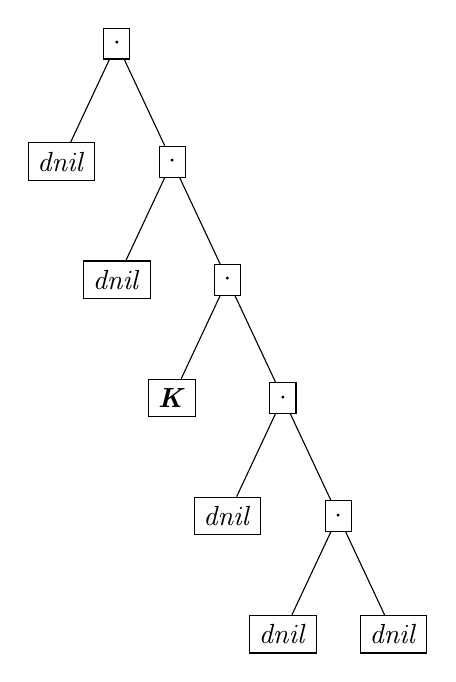
\begin{tikzpicture}[sibling distance=4em,
  every node/.style = {shape=rectangle,
    draw, align=center,
    top color=white, bottom color=white}]]
  \node {$\cdot$}
    child { node {\textit{dnil}} }
    child { node {$\cdot$}
      child { node {\textit{dnil}}}
      child { node {$\cdot$} 
	child { node {\textit{\textbf{K}}} } 
	child { node {$\cdot$} 
		child { node {\textit{dnil}} }
		child { node {$\cdot$} 
			child { node {\textit{dnil}} }
			child { node {\textit{dnil}} } } } } };
\end{tikzpicture} \textbf{\textit{:: []}}
\end{center}
Then we can transform the \textit{command} following our previous definition.
Then we should extract the result from the accumulated one-variable environment.
For example the original \textit{program} will write the value to the variable \textbf{D} as the output, then our transformed \textit{program} should have the same out put.
However after the execution of the \textit{command}, we will get an accumulated one-variable environment, and we will write the variable \textit{zero} as out put.
Thus, the \textit{command} will extract the value to the variable and replace the whole variable \textit{zero} with the output.
\begin{center}
\begin{tikzpicture}[sibling distance=4em,
  every node/.style = {shape=rectangle,
    draw, align=center,
    top color=white, bottom color=white}]]
  \node {$\cdot$}
    child { node {\textit{A}} }
    child { node {$\cdot$}
      child { node {\textit{B}}}
      child { node {$\cdot$} 
	child { node {\textit{C}} } 
	child { node {$\cdot$} 
		child { node {\textit{\textbf{D}}} }
		child { node {$\cdot$} 
			child { node {\textit{E}} }
			child { node {\textit{dnil}} } } } } };
\end{tikzpicture} \textbf{\textit{:: []}}
$\Longrightarrow$ \textbf{D} \textbf{\textit{:: []}} 
\end{center}
\begin{code}[fontsize=\small]
p-multi-one-h : {m : ℕ}(ini : E 1) → (inp : E 1) → (pos : Fin m) → ℕ → E 1
p-multi-one-h ini inp zero n = cons inp (e-var (fromℕ n) ini)
p-multi-one-h ini inp (suc pos) n = cons nil (p-multi-one-h ini inp pos (suc n))

p-multi-one : {n : ℕ} → P n → P 1
p-multi-one {n}(prog x c y)
= prog zero ((zero := p-multi-one-h (dtoE {1}
                                          (head (env-multi-one (initialVec {n}))))
                                    (var zero) x (suc zero))
              →→ c-multi-one c
              →→ (zero := e-multi-one (var y)))
       zero
\end{code}
We must prove our transformation of the \textit{program} is correct.
We can divide our transformed \textit{program} into three parts: constructing the environment, the transformed \textit{command} and extracting the output.
We should prove their correctness separately at first.
\begin{code}[fontsize=\small]
p-lemma₁ : {n : ℕ}{x : Fin n}{d : D}
         → ((zero := p-multi-one-h (dtoE {1} (head (env-multi-one (initialVec {n}))))
                     (var zero) x (suc zero))
           ⊢ d ∷ [] ⇒  env-multi-one (updateE x d (initialVec {n})))
p-lemma₁ = ?

p-lemma₂ : {n : ℕ}{y : Fin n}{env : Vec D n}
         → ((zero := e-multi-one (var y)) ⊢ env-multi-one env ⇒ (dlookup y env ∷ []))
p-lemma₂ = ?
\end{code}
Finally we should prove the correctness of the whole \textit{program} transformation.
\begin{code}[fontsize=\small]
p-multi-one-ok : {n : ℕ} → {p : P n} → {d₁ d₂ : D}
                 → ExecP p d₁ d₂
                 → ExecP (p-multi-one p) d₁ d₂
p-multi-one-ok = ?
\end{code}
\subsection{Proof the Undecidability of the Halting Problem}
As we can prove that the WHILE program has the same computation ability with \textit{WHILE-I} program which has only one variable,
we can conclude that our universal WHILE program can simulate the WHILE program with arbitrary variables, 
furthermore, we can conclude that we can prove the undecidability of the halting problem in the system we built.
Here gives an example on how could we use the transformation step to execute the arbitrary WHILE program using one variable, 
for \textit{p} $\in$ \md{P} $n$ and \textit{input}, \textit{output} $\in$ \md{D}, if we want to use our universal WHILE program to simulate $p(input)$,
then we should transform $p$ to $p$-$I$ which has only one variable by our predefined transformation function.
And we know that $p(input)$ yielding $output$ implies that $p$-$I(input)$ yielding $output$ by the proof of correctness of the transformation function.
And by the proof of the correctness of the universal WHILE program we know that $p$-$I(input)$ yielding $output$ implies that $u(\lfloor p$-$I\rfloor \cdot input)$ yielding $output$.
Thus we can conclude that for \textit{p} $\in$ \md{P} $n$ and \textit{input}, \textit{output} $\in$ \md{D}, $p(input)$ yielding $output$ implies $u(\lfloor p$-$I\rfloor \cdot input)$ yielding $output$ which means universal WHILE program can simulate the WHILE program has arbitrary variables.\\
Thus for the proof of Halting problem, we can say that for \textit{p} $\in$ \md{P} $n$, \textit{h} can decide the Halting problem implies \textit{false}.
\begin{code}[fontsize=\small]
halt-contradiction-arb : ∀ {m} {h : P m}
                   → (∀ {n : ℕ} → ∀ {p : P n} → ∀ {inp : D}
                      → (Σ D (ExecP p inp) → ExecP h ((codeP p) ∙ inp) dtrue)
                      ×' ((∀ {out : D} → ExecP p inp out → ⊥)
                          → ExecP h ((codeP p) ∙ inp) dfalse))
                   → ⊥
halt-contradiction-arb {m} {h} p = halt-contradiction {p-multi-one {m} h}
                                   (λ {n : ℕ} {p₁ : P n} {inp : D}
                                   → (λ x → p-multi-one-ok {m} {h}
                                                           {(codeP p₁) ∙ inp}
                                                           {dtrue}
                                                           (proj₁ (p {n} {p₁} {inp}) x))
                                   ,'(λ x → p-multi-one-ok {m} {h}
                                                           {(codeP p₁) ∙ inp}
                                                           {dfalse}
                                                           (proj₂ (p {n} {p₁} {inp})
                                                                  (λ y → x y))))
\end{code}
\section{Conclusion}
In this paper, we construct a self-interpret system using Agda, following the definition by \textit{Neil D. Jones} in 1997 \cite{jones_computability_1997}.
We prove the correctness of our system, and the property of Turing-completeness and Turing-equivalence among this system.
Then we pick a kind of particular programs, the programs have one one variable, and prove the undecidability of the Halting problem using the interpretation under the program that has only one variable.
Furthermore, we construct a transformation function which will transform the program that has arbitrary variables to the program that has only one variable.
We prove the correctness of the transformation, which means in our system the program has many variables has the same computation power compare to some programs that has only one variable.
Finally, we can use our transformation function to prove the undecidability of the Halting problem in our system.\\

\bibliographystyle{alpha}
\bibliography{local}{}

\end{document}